% Provenance (never printed): see sources/outline_sources.md (Year 3: the
% structure of the Galaxy; the rotation curve and dark matter; galaxy types;
% the distance ladder, Hubble's law recalled from the physics books).
% Brief: sources/book5/BRIEFS.md, ch. 29. Curves from figdata/bachelor-3/
% rotation_curve.py (the circular velocity curve of Eilers et al. 2019 with the
% Pouliasis et al. 2017 Model I baryons and an NFW halo fitted to it) and
% distance_ladder.py (the OGLE-IV Cepheids of the Large Magellanic Cloud, CDS
% J/AcA/65/297, and the ranges of the rungs). Exercise and problem values in the
% Book 5 scratch calculator calc/ch29.py. The survey of Part I of the problem and
% the galaxies of the exercises are invented.
\chapter{A Via Láctea e as galáxias}\label{ch:b3:milky-way-galaxies}

No Sistema Solar, os planetas distantes do Sol movem-se devagar: Mercúrio
circula-o a \qty{47.4}{km.s^{-1}}, Netuno a \qty{5.4}{km.s^{-1}}, como
exige a terceira lei de Kepler de corpos presos a uma única massa central. As estrelas
da Galáxia não se comportam assim. Medidas a partir dos movimentos de mais de
vinte mil gigantes vermelhas, a velocidade de suas órbitas circulares é
\qty{227}{km.s^{-1}} a \qty{5}{kpc} do centro, \qty{229}{km.s^{-1}}
no Sol e ainda \qty{198}{km.s^{-1}} a \qty{25}{kpc}, onde quase não restam
estrelas nem gás. Se a massa que vemos fosse tudo o que existe, as estrelas externas
seriam muito mais lentas. Algo invisível as sustenta. Este capítulo descreve a Galáxia
em que vivemos, pesa-a a partir de sua rotação, classifica as
outras galáxias em tipos e percorre a cadeia de métodos pelos quais suas
distâncias, e a expansão do Universo, são medidas.
% ledger: planet:Mercury.vorb, planet:Neptune.vorb, eilers19:vc, eilers19:table1

\begin{recall}
A Via Láctea, o efeito Doppler, as leis de Kepler, o teorema de Newton sobre a
atração de uma casca esférica, a matéria escura, os buracos negros e seu
raio de Schwarzschild, as supernovas, as anãs brancas, a linha de 21~cm do
hidrogênio atômico e a lei de Hubble estão nos livros de física. A paralaxe anual,
o parsec, o fluxo e a luminosidade, as magnitudes aparente e absoluta, o
módulo de distância, as bandas fotométricas e o índice de cor estão no
volume do primeiro~ano, em seu capítulo sobre telescópios e fotometria. O
meio interestelar e sua poeira estão no volume do segundo~ano, em seu capítulo
sobre o meio interestelar e a formação estelar.
\end{recall}

\section{A estrutura da Galáxia}\label{sec:b3:milky-way-galaxies:structure}

Vista da Terra, a Galáxia é a Via Láctea: uma faixa de luz ao redor
de todo o céu, cortada por faixas escuras de poeira e mais brilhante em direção
à constelação de Sagitário, onde fica seu centro. A faixa é o disco em que
o Sol está, visto de perfil por dentro.

\begin{omfigure}
\centering
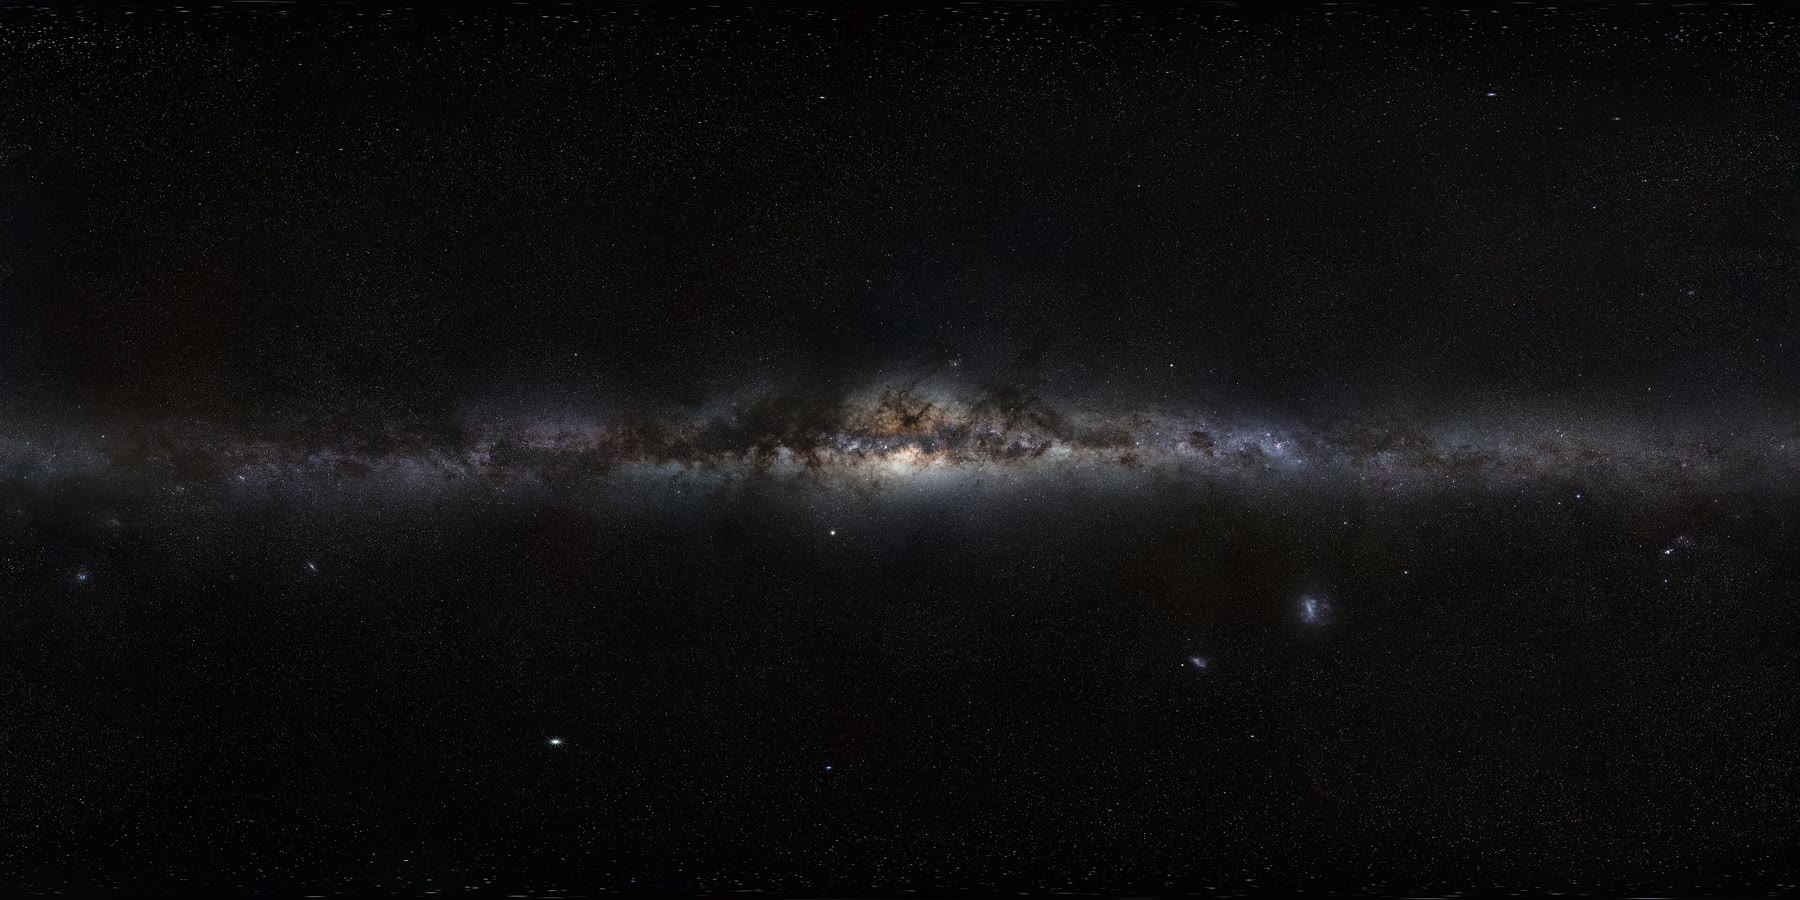
\includegraphics[width=0.96\linewidth]{images/book5/b3-milky-way-panorama.jpg}
\par\smallskip{\small O céu inteiro numa só imagem, projetado de modo que o
plano da Galáxia atravesse o meio e seu centro fique no
centro da imagem. A faixa é o disco visto por dentro; as faixas escuras são
poeira no disco, ocultando as estrelas atrás dele; o bojo central
incha em torno do centro. As duas pequenas manchas abaixo da faixa, do
lado direito, são as Grandes e Pequenas Nuvens de Magalhães, duas galáxias satélites;
a mancha tênue abaixo da faixa, perto da borda esquerda, é a galáxia de Andrômeda.
Fotografia ESO/S.~Brunier, CC BY~4.0.}\label{fig:b3:milky-way-galaxies:panorama}
\end{omfigure}
% ledger: photo:b3-milky-way-panorama, mcconn12:local-group

\begin{definition}[Disco galáctico, disco espesso, bojo galáctico e halo estelar]\label{def:b3:milky-way-galaxies:structure}
O \emph{disco galáctico}\index{disco galáctico} é o componente achatado da
Galáxia, formado por estrelas, gás e poeira em órbitas quase circulares em torno de seu
centro; sua densidade cai aproximadamente de forma exponencial com a altura acima de seu
plano médio e com a distância ao centro, ao longo de uma altura de escala e de uma
comprimento de escala. O \emph{disco espesso}\index{disco espesso} é um segundo, mais antigo,
componente de disco, de maior altura de escala e menor massa. O
\emph{bojo galáctico}\index{bojo galáctico} é a concentração central de
estrelas que se projeta para fora do disco. O \emph{halo estelar}\index{halo estelar}
é o componente esparso, aproximadamente esferoidal, de estrelas velhas e
aglomerados globulares que envolve o disco e o bojo.
\end{definition}

A Galáxia é uma espiral barrada. Na vizinhança do Sol, o disco fino tem
altura de escala de cerca de \qty{300}{pc}, e o \omterm{def:b3:milky-way-galaxies:structure}{disco espesso}, de cerca de
\qty{900}{pc}; seus comprimentos de escala são de cerca de \qty{2.6}{kpc} e
\qty{2.0}{kpc}. O \omterm{def:b3:milky-way-galaxies:structure}{disco espesso} contém cerca de \num{6e9} massas solares,
cerca de um quinto do disco fino. Visto de lado, o bojo tem a forma de uma caixa
ou de um amendoim: é a parte interna engrossada de uma barra de estrelas de cerca de
\qty{5}{kpc} de meio-comprimento, cujo eixo longo forma um ângulo de
\ang{27} com a linha que vai do Sol ao centro. O \omterm{def:b3:milky-way-galaxies:structure}{halo estelar} contém
apenas cerca de um por cento das estrelas. Ao todo, as estrelas da Galáxia
pesam cerca de \num{5e10} massas solares.
% ledger: bhg16:structure

\begin{omfigure}
\centering
\begin{tikzpicture}[x=0.17cm, y=0.17cm, font=\scriptsize]
% edge-on view
\begin{scope}
\fill[omProp!8] (0,0) circle (17);
\draw[omProp!60, densely dotted] (0,0) circle (17);
\fill[black!12] (0,0) ellipse (15 and 2.4);
\fill[black!30] (0,0) ellipse (15 and 0.8);
\fill[black!45] (-3.2,0) .. controls (-3.4,2.3) and (-1.2,2.0) .. (0,1.4)
  .. controls (1.2,2.0) and (3.4,2.3) .. (3.2,0)
  .. controls (3.4,-2.3) and (1.2,-2.0) .. (0,-1.4)
  .. controls (-1.2,-2.0) and (-3.4,-2.3) .. (-3.2,0) -- cycle;
\foreach \p in {(-10,9),(6,12),(12,-7),(-6,-13),(-13,-4),(3,-9),(12,8)}
  \fill[omProp] \p circle (0.35);
\fill[ocYellow, draw=black] (-8.2,0.15) circle (0.55);
\node[anchor=south] at (-8.2,0.9) {Sol};
\draw[|<->|] (0,-4.6) -- node[below] {$R_0 \approx \qty{8.2}{kpc}$} (-8.2,-4.6);
\node[anchor=west] at (15.3,0) {disco fino};
\node[anchor=west] at (13.2,2.8) {disco espesso};
\draw[->] (4.6,4.6) node[anchor=south west, inner sep=1pt] {bojo} -- (2.4,1.7);
\node[omProp!80!black] at (-11,13.5) {halo estelar};
\node at (0,-19.5) {(a) visto de perfil};
\end{scope}
% face-on view
\begin{scope}[xshift=7.6cm]
\fill[omProp!8] (0,0) circle (17);
\draw[omProp!60, densely dotted] (0,0) circle (17);
\fill[black!12] (0,0) circle (15);
\foreach \a in {0,180} {
  \draw[line width=1.6pt, black!40, rotate=\a+63]
    plot[domain=0:3.9, samples=50] ({5*exp(0.25*\x)*cos(\x r)}, {5*exp(0.25*\x)*sin(\x r)});
}
\fill[black!45, rotate=63] (0,0) ellipse (5 and 1.5);
\draw[dashed] (0,0) circle (8.2);
\fill[ocYellow, draw=black] (0,-8.2) circle (0.55);
\node[anchor=north] at (0,-8.9) {Sol};
\draw[dotted, thick] (0,0) -- (0,-8.2);
\draw[thick, ->] (0,0) ++(25:16) arc (25:-25:16);
\node[anchor=west] at (17.3,0) {rotação};
\node[anchor=west, fill=black!12, inner sep=1pt] at (3.4,3.4) {barra};
\draw[|-|] (6,-15.5) -- node[below] {\qty{5}{kpc}} (11,-15.5);
\node at (0,-19.5) {(b) visto do polo galáctico norte};
\end{scope}
\end{tikzpicture}
\par\smallskip{\small Esquema da Galáxia, em escala quanto às suas principais
dimensões. (a)~Visto de perfil: o disco fino (faixa escura), o \omterm{def:b3:milky-way-galaxies:structure}{disco espesso} (faixa
clara), o bojo em forma de caixa e o \omterm{def:b3:milky-way-galaxies:structure}{halo estelar} com seus
aglomerados globulares (pontos laranja); o Sol está no disco, a cerca de \qty{8.2}{kpc}
do centro e a cerca de \qty{25}{pc} acima do plano médio (pequeno demais para
aparecer). (b)~Visto do polo galáctico norte: a barra, com cerca de
\qty{5}{kpc} de meio-comprimento, inclinada de \ang{27} em relação à linha que vai do Sol
ao centro (pontilhada); o círculo solar (tracejado); braços espirais desenhados
de forma esquemática; a Galáxia gira no sentido horário nesta vista.}\label{fig:b3:milky-way-galaxies:sketch}
\end{omfigure}
% ledger: bhg16:structure, gravity19:r0

\begin{definition}[População estelar]\label{def:b3:milky-way-galaxies:populations}
Uma \emph{população estelar}\index{população estelar} é um grupo de estrelas
de uma galáxia que compartilham uma faixa de idades, de composições químicas e de
órbitas. As estrelas jovens do disco fino, ricas em elementos mais pesados que
o hélio e em órbitas quase circulares, são tradicionalmente chamadas
população~I; as estrelas velhas do halo e dos aglomerados globulares, pobres
em elementos pesados e em órbitas de grandes movimentos aleatórios com pouca
rotação líquida, população~II.
\end{definition}

O \omterm{def:b3:milky-way-galaxies:structure}{disco espesso} fica numa posição intermediária: suas estrelas são, em sua maioria, mais velhas que as
do disco fino e, para um dado teor de ferro, mais ricas nos elementos leves que os astrônomos
chamam de elementos alfa, medidos em relação ao ferro. O \omterm{def:b3:milky-way-galaxies:structure}{halo estelar} é
um registro fóssil: grande parte dele foi montada a partir de pequenas galáxias que caíram na
Galáxia e foram despedaçadas por suas marés, e alguns de seus fluxos de estrelas
ainda podem ser acompanhados
pelo céu.
% ledger: bhg16:populations

\begin{definition}[Coordenadas galácticas]\label{def:b3:milky-way-galaxies:coordinates}
As \emph{coordenadas galácticas}\index{coordenadas galácticas} de uma direção
são sua \emph{latitude galáctica} $b$, o ângulo medido a partir do plano galáctico
(positiva em direção ao polo galáctico norte), e sua \emph{longitude
galáctica} $\ell$, medida no plano a partir da direção do
centro galáctico ($\ell = 0$) até $\ell = \ang{90}$, a direção
para a qual a rotação da Galáxia leva o Sol. O plano foi
definido em 1958 como o plano principal do hidrogênio atômico da Galáxia;
o polo galáctico norte situa-se na ascensão reta \ang{192.25}
($12^\mathrm{h}49^\mathrm{m}$) e declinação \ang{27.4} (equinócio
1950).
\end{definition}
% ledger: liu11:galactic, reid20:sgra

O Sol não está exatamente no plano: ele se situa cerca de \qty{25}{pc} ao norte dele.
Sua distância ao centro, $R_0$, foi por muito tempo o número mais incerto da
astronomia galáctica. Hoje ela é medida geometricamente: a estrela S2 orbita
o buraco negro central da Galáxia em uma órbita de \num{16} anos, cujos
tamanho angular no céu e velocidade ao longo da linha de visada, acompanhados
por 27 anos, fornecem diretamente a distância ao centro:
$R_0 = \qty{8178}{pc}$, com erro estatístico de \qty{13}{pc} e um
sistemático de \qty{22}{pc}. Uma revisão de todos os métodos fornece
$R_0 = \qty[separate-uncertainty=true]{8.2 \pm 0.1}{kpc}$.
% ledger: bhg16:structure, gravity19:r0

\section{Rotação e halo de matéria escura}\label{sec:b3:milky-way-galaxies:rotation}

\begin{definition}[Padrão local de repouso]\label{def:b3:milky-way-galaxies:lsr}
O \emph{padrão local de repouso}\index{padrão local de repouso} (LSR) é
o referencial que se move na órbita circular em torno do centro galáctico que
passa pela posição atual do Sol. As velocidades de estrelas e gás próximos
são dadas em relação a ele.
\end{definition}

O Sol se move em relação ao LSR com cerca de \qty{10}{km.s^{-1}} em direção ao
centro galáctico, \qty{11}{km.s^{-1}} no sentido da rotação e
\qty{7}{km.s^{-1}} em direção ao polo galáctico norte: um pequeno movimento peculiar
somado a uma órbita com velocidade $V_0$ de algumas centenas de quilômetros
por segundo. Vista da Terra, a fonte de rádio no centro da
Galáxia desloca-se ao longo do plano galáctico em \qty{6.411}{mas} por ano; quase
todo esse deslocamento é o reflexo da órbita do Sol e fornece a
velocidade total do Sol em torno do centro, \qty[separate-uncertainty=true]{248 \pm 3}{km.s^{-1}}
(\cref{exo:b3:milky-way-galaxies:2}).
% ledger: bhg16:lsr, reid20:sgra

\begin{definition}[Curva de rotação; constantes de Oort]\label{def:b3:milky-way-galaxies:rotation-curve}
A \emph{curva de rotação}\index{curva de rotação} de uma galáxia de disco é a
velocidade $V(R)$ de uma órbita circular em seu plano em função da
distância $R$ ao seu centro. Para a Galáxia, com $V_0 = V(R_0)$ e
$V'_0 = \mathrm{d}V/\mathrm{d}R$ em $R_0$, as \emph{constantes de
Oort}\index{constantes de Oort} são
\[
A = \frac12\left(\frac{V_0}{R_0} - V'_0\right), \qquad
B = -\frac12\left(\frac{V_0}{R_0} + V'_0\right).
\]
\end{definition}

$A$ mede o cisalhamento da rotação do disco e $B$ sua vorticidade: em um
disco que gira como corpo rígido $V'_0 = V_0/R_0$ e $A = 0$; em uma \omterm{def:b3:milky-way-galaxies:rotation-curve}{curva de
rotação} plana $A = -B$. A diferença entre elas é a velocidade angular do LSR,
$A - B = V_0/R_0 = \omega_0$, e a soma delas é a inclinação, $A + B = -V'_0$.

\begin{theorem}[Fórmulas de Oort]\label{thm:b3:milky-way-galaxies:oort}
Uma estrela a uma distância $d \ll R_0$ do Sol, no plano galáctico, na
longitude $\ell$, em órbita circular, tem em relação ao LSR a velocidade radial
$v_r$ e a velocidade transversal $v_t$ (positiva no
sentido de crescimento de $\ell$)
\[
v_r = A\,d\sin 2\ell, \qquad v_t = d\,(A\cos 2\ell + B),
\]
em primeira ordem em $d/R_0$.
\end{theorem}

\begin{proof}
Seja $\omega(R) = V(R)/R$ a velocidade angular da órbita em $R$. Toma-se o
centro galáctico como origem, o Sol à distância $R_0$, e seja a estrela à
distância $R$ do centro, sua posição vista do centro fazendo o ângulo
$\theta$ com a do Sol. Projetando a velocidade da estrela
$\omega R$ e a velocidade do LSR $\omega_0 R_0$ na linha de visada, uma
pequena trigonometria no triângulo Sol--estrela--centro (a lei dos senos
fornece $R\sin(\ell + \theta) = R_0\sin\ell$) o resultado exato
$v_r = R_0\,[\omega(R) - \omega_0]\sin\ell$. Analogamente, na direção
perpendicular à linha de visada,
$v_t = R_0\,[\omega(R) - \omega_0]\cos\ell - \omega(R)\,d$. Para uma estrela
próxima, $\omega(R) - \omega_0 \approx \omega'_0\,(R - R_0)$ e
$R - R_0 \approx -d\cos\ell$. Então
$v_r \approx -R_0\omega'_0\,d\cos\ell\sin\ell = -\tfrac12 R_0\omega'_0\,
d\sin 2\ell$ e, mantendo os termos de primeira ordem,
$v_t \approx -R_0\omega'_0\,d\cos^2\ell - \omega_0 d$. Com
$\omega'_0 = V'_0/R_0 - V_0/R_0^2$, $-\tfrac12 R_0\omega'_0 = A$ e
$-R_0\omega'_0\cos^2\ell - \omega_0 = A(1 + \cos 2\ell) - (A - B) =
A\cos 2\ell + B$.
\end{proof}

As velocidades radiais das estrelas próximas variam, portanto, como $\sin 2\ell$ ao
longo do céu, e os seus movimentos próprios, como $\cos 2\ell$ em torno de uma média fixada por $B$.
A partir dos movimentos próprios e das paralaxes de \num{304267} estrelas do primeiro
catálogo Gaia, a uma distância típica de \qty{230}{pc}, as \omterm{def:b3:milky-way-galaxies:rotation-curve}{constantes de Oort}
são $A = \qty[separate-uncertainty=true]{15.3 \pm 0.4}{km.s^{-1}.kpc^{-1}}$
e $B = \qty[separate-uncertainty=true]{-11.9 \pm 0.4}{km.s^{-1}.kpc^{-1}}$.
Dois outros termos que um disco axissimétrico não teria, chamados $C$
e $K$, resultaram em cerca de \qty{-3}{km.s^{-1}.kpc^{-1}}: o disco local é
agitado pela barra e pelos braços espirais.
% ledger: bovy17:oort

\subsection*{A curva de rotação a partir da linha de 21 cm}

O hidrogênio atômico preenche o disco e emite a linha de 21 cm, em
\qty{1420.405751}{MHz}; as ondas de rádio atravessam a poeira que oculta o
disco distante em comprimentos de onda visíveis. Ao longo de uma linha de visada
no plano, cada nuvem de gás acrescenta a sua linha com o desvio Doppler de
sua velocidade radial, e o perfil da linha é um espectro de
velocidades. Dentro do círculo solar, uma velocidade se destaca.
% ledger: nrao:hi-line

\begin{theorem}[Método do ponto de tangência]\label{thm:b3:milky-way-galaxies:tangent}
Suponha-se que o gás se mova em órbitas circulares com velocidade angular $\omega(R)$ que
diminui para fora. Ao longo de uma linha de visada na longitude
$0 < \ell < \ang{90}$, a velocidade radial em relação ao PLR é maior
no ponto de tangência, onde a linha de visada é tangente a uma órbita, em
$R = R_0\sin\ell$, e o seu maior valor é
\[
v_\mathrm{max} = V(R_0\sin\ell) - V_0\sin\ell .
\]
\end{theorem}

\begin{proof}
Pela demonstração das fórmulas de Oort, o gás à distância $R$ do centro na
linha de visada tem $v_r = R_0\,[\omega(R) - \omega_0]\sin\ell$. Com
$\sin\ell > 0$ e $\omega$ decrescente, $v_r$ é maior onde $R$ é
menor. Ao longo da linha de visada, $R$ é menor no pé da
perpendicular traçada a partir do centro, onde $R = R_0\sin\ell$. Ali
$R_0\,\omega(R)\sin\ell = \omega(R)\,R = V(R)$ e
$R_0\,\omega_0\sin\ell = V_0\sin\ell$.
\end{proof}

\begin{omfigure}
\centering
\begin{tikzpicture}[scale=0.95, font=\small]
\coordinate (C) at (0,0);
\coordinate (S) at (0,-4);
\coordinate (T) at (-1.970,-1.653);
\draw[dashed, black!50] (C) circle (4);
\draw[dashed, omDef!70] (C) circle (2.571);
\fill (C) circle (2pt) node[anchor=south west] {Centro Galáctico};
\fill[ocYellow, draw=black] (S) circle (3pt);
\node[anchor=north] at (0,-4.15) {Sol};
\draw[thick] (S) -- ($(S)!2.25!(T)$) node[anchor=south east, fill=white, inner sep=1pt] {linha de visada};
\draw[dotted, thick] (C) -- (S);
\draw[thick, omThm] (C) -- node[anchor=north west, fill=white, inner sep=1pt, pos=0.45] {$R_0\sin\ell$} (T);
\fill[omThm] (T) circle (2pt);
\node[anchor=north east, omThm, fill=white, inner sep=1pt] at ($(T)+(-0.05,-0.08)$) {ponto de tangência};
\draw[->, very thick, omDef] (T) -- ++(-0.643*1.3, 0.766*1.3) node[anchor=south west, fill=white, inner sep=1pt] {$V(R)$};
\draw[->, very thick, black!70] (S) -- ++(-1.4,0) node[anchor=north] {$V_0$};
\draw (0,-3.2) arc (90:130:0.8);
\node at (-0.30,-2.85) {$\ell$};
\node[anchor=west] at (0.1,-2.2) {$R_0$};
\node[black!60, anchor=west] at (2.9,-2.9) {círculo solar};
\end{tikzpicture}
\par\smallskip{\small O método do ponto de tangência, visto do polo galáctico
norte. Ao longo de uma linha de visada na longitude $\ell$, o gás mais próximo
do centro fica no ponto de tangência, em $R = R_0\sin\ell$ (em vermelho); sua
velocidade orbital $V(R)$ é ao longo da linha de visada, e o
velocidade radial ali é a maior que o perfil da linha mostra. Cada
longitude fornece um ponto da \omterm{def:b3:milky-way-galaxies:rotation-curve}{curva de rotação} dentro do círculo solar.}\label{fig:b3:milky-way-galaxies:tangent}
\end{omfigure}

A velocidade mais alta em cada perfil de 21 cm fornece, assim, $V$ em
$R_0\sin\ell$, e uma varredura de longitudes de \ang{0} a \ang{90} fornece
a \omterm{def:b3:milky-way-galaxies:rotation-curve}{curva de rotação} desde o centro até o Sol. Além do
círculo solar, nenhuma linha de visada é tangente a uma órbita, e o método falha:
ali, a distância de cada traçador precisa ser medida, além da sua
velocidade. Desde 2014, um satélite mediu as paralaxes de mais de um
bilhão de estrelas, e a \omterm{def:b3:milky-way-galaxies:rotation-curve}{curva de rotação} externa é agora traçada por estrelas.
% ledger: nrao:hi-line, gaia:dr3

\begin{omfigure}
\centering
\begin{tikzpicture}
\begin{axis}[width=0.90\linewidth, height=0.52\linewidth,
  xmin=0, xmax=26, ymin=0, ymax=265,
  xlabel={distância do centro galáctico $R$ (kpc)}, ylabel={velocidade circular (\unit{km.s^{-1}})},
  tick label style={font=\scriptsize}, label style={font=\small},
  legend style={font=\scriptsize, at={(0.5,-0.16)}, anchor=north, legend columns=4, draw=none, cells={anchor=west}, /tikz/every even column/.append style={column sep=1em}}]
\addplot[thin, black!40, dashed, forget plot] coordinates {(8.122,0) (8.122,265)};
\node[font=\scriptsize, anchor=south west, rotate=90] at (axis cs:7.9,4) {Sol};
\addplot[only marks, mark=*, mark size=1.1pt, black, error bars/.cd, y dir=both, y explicit]
  table[x=R, y=vc, y error minus=sig_lo, y error plus=sig_hi] {figdata/out/bachelor-3-rotation_curve-data.dat};
\addlegendentry{medida}
\addplot[very thick, omDef] table[x=R, y=v_tot] {figdata/out/bachelor-3-rotation_curve-model.dat};
\addlegendentry{modelo total}
\addplot[thick, black!55] table[x=R, y=v_bar] {figdata/out/bachelor-3-rotation_curve-model.dat};
\addlegendentry{todos os bárions}
\addplot[thick, dashed, red!70!black] table[x=R, y=v_halo] {figdata/out/bachelor-3-rotation_curve-model.dat};
\addlegendentry{halo escuro}
\addplot[densely dotted, thick, omProp] table[x=R, y=v_bulge] {figdata/out/bachelor-3-rotation_curve-model.dat};
\addlegendentry{bojo}
\addplot[dashdotted, thick, omMeth] table[x=R, y=v_thin] {figdata/out/bachelor-3-rotation_curve-model.dat};
\addlegendentry{disco fino}
\addplot[densely dashed, thick, violet!70!black] table[x=R, y=v_thick] {figdata/out/bachelor-3-rotation_curve-model.dat};
\addlegendentry{disco espesso}
\end{axis}
\end{tikzpicture}
\par\smallskip{\small A \omterm{def:b3:milky-way-galaxies:rotation-curve}{curva de rotação} da Galáxia. Pontos: a velocidade circular
medida a partir de gigantes vermelhas entre 5 e \qty{25}{kpc} (Eilers
e outros, 2019), com as suas barras de erro. Curvas: as velocidades que o
bojo, o disco fino e o \omterm{def:b3:milky-way-galaxies:structure}{disco espesso} de um modelo de massa publicado daria
isoladamente (Pouliasis e outros, 2017), a sua combinação (cinza) e
o halo escuro ajustado aqui às medidas (vermelho tracejado), que assume
o lugar dos bárions além de \qty{14}{kpc}; eles se somam em quadratura ao
total (azul). Os \qty{5}{kpc} internos, onde a barra torna as órbitas
bem distantes de circulares, ficam de fora da medida.}\label{fig:b3:milky-way-galaxies:rotation}
\end{omfigure}
% ledger: eilers19:table1, eilers19:vc, eilers19:halo, pouliasis17:model1, data:b5-rotation-fit

A curva da figura acima foi medida a partir das posições, distâncias
e velocidades de mais de vinte e três mil gigantes vermelhas luminosas,
com a equação da hidrodinâmica estelar que relaciona os movimentos médios
de uma população de estrelas à gravidade que as mantém (a equação de Jeans).
No Sol, obtém-se $V_0 = \qty{229.0}{km.s^{-1}}$, com uma incerteza sistemática
de dois a cinco por cento; além disso, ela decresce suavemente, em
\qty[separate-uncertainty=true]{1.7 \pm 0.1}{km.s^{-1}} por quiloparsec. Ela
não cai como exige a massa visível.
% ledger: eilers19:vc

\subsection*{Pesando a Galáxia}

A gravidade de um disco não é a de uma esfera, mas a curva de velocidade
de um modelo de massa calcula-se facilmente quando cada componente tem um potencial em
forma fechada. Os potenciais no plano abaixo são os de um modelo publicado
das estrelas da Galáxia.

\begin{proposition}[Velocidades circulares de três modelos de massa]\label{prop:b3:milky-way-galaxies:models}
No plano $z = 0$, a velocidade circular $V^2 = R\,\partial\Phi/\partial R$
é, para
\begin{itemize}
\item uma esfera de Plummer de massa $M$ e raio do núcleo $b$, de potencial
  $\Phi = -GM/\sqrt{r^2 + b^2}$:
  \[ V^2 = \frac{GMR^2}{(R^2 + b^2)^{3/2}}\,; \]
\item um disco de Miyamoto--Nagai de massa $M$, comprimento de escala $a$ e
  altura de escala $b$, de potencial
  $\Phi = -GM\big/\sqrt{R^2 + \bigl(a + \sqrt{z^2 + b^2}\,\bigr)^2}$:
  \[ V^2 = \frac{GMR^2}{\bigl(R^2 + (a + b)^2\bigr)^{3/2}}\,; \]
\item um halo de Navarro--Frenk--White de densidade
  $\rho = \rho_0\big/\bigl[x(1 + x)^2\bigr]$, $x = r/R_s$: a massa dentro de $r$
  é $M(r) = 4\pi\rho_0R_s^3\bigl[\ln(1 + x) - x/(1 + x)\bigr]$ e
  $V^2 = GM(r)/r$.
\end{itemize}
Para vários componentes, somam-se os quadrados das velocidades.
\end{proposition}

\begin{proof}
Para os dois primeiros, deriva-se o potencial em relação a $R$ em
$z = 0$. Para o halo, integra-se $4\pi r^2\rho$ de 0 a $r$: com
$u = 1 + x'$, $\int_0^x x'\,\mathrm{d}x'/(1 + x')^2 =
\int_1^{1+x}(u - 1)\,\mathrm{d}u/u^2 = \ln(1 + x) + 1/(1 + x) - 1$; uma
massa esférica atua sobre uma órbita em $r$ como se toda a sua massa dentro de $r$ estivesse
no centro (teorema de Newton). Os potenciais somam-se, daí as suas
derivadas radiais.
\end{proof}

O modelo usado na figura tem um bojo de Plummer de
\num{1.07e10} massas solares com $b = \qty{0.3}{kpc}$, um disco fino e um
\omterm{def:b3:milky-way-galaxies:structure}{disco espesso} de \num{3.94e10} massas solares cada, com $(a, b) =
(\qty{5.3}{kpc}, \qty{0.25}{kpc})$ e $(\qty{2.6}{kpc}, \qty{0.8}{kpc})$.
Com $G = \qty{4.301e-6}{kpc.(km.s^{-1})^2}$ por massa solar, suas estrelas
sozinhas dariam ao Sol uma velocidade orbital de \qty{184}{km.s^{-1}}, e
a uma estrela a \qty{20}{kpc}, uma de \qty{134}{km.s^{-1}}; as velocidades medidas são
229 e \qty{200}{km.s^{-1}}. Um halo ajustado às medidas, com as
estrelas mantidas fixas, tem $R_s = \qty{14.75}{kpc}$ e
$\rho_0 = \num{1.06e7}$ massas solares por quiloparsec cúbico, o mesmo que
o halo que seus autores ajustaram ($R_s = \qty[separate-uncertainty=true]{14.8 \pm 0.4}{kpc}$,
$\rho_0 = \qty[separate-uncertainty=true]{1.06 \pm 0.09 e7}{}$ massas solares
por quiloparsec cúbico). O halo domina além de cerca de \qty{14}{kpc}.
% ledger: pouliasis17:model1, data:b5-rotation-fit, eilers19:halo, eilers19:table1, const:G, sun:mass, iau:parsec

\begin{definition}[Halo de matéria escura]\label{def:b3:milky-way-galaxies:halo}
O \emph{halo de matéria escura}\index{halo de matéria escura} de uma galáxia é a
distribuição de matéria escura aproximadamente esférica em que estão imersas suas estrelas e seu gás,
muito maior e mais massiva do que suas componentes visíveis,
e inferida a partir de sua gravidade: da \omterm{def:b3:milky-way-galaxies:rotation-curve}{curva de rotação}, dos movimentos
de galáxias satélites e de estrelas do halo, e da curvatura da luz.
\end{definition}

\begin{theorem}[Massa dentro de um raio]\label{thm:b3:milky-way-galaxies:enclosed}
Para uma distribuição esférica de massa, a velocidade circular no raio $r$
fornece a massa dentro dele, $M(r) = rV^2/G$. Uma \omterm{def:b3:milky-way-galaxies:rotation-curve}{curva de rotação} plana,
$V = $ constante, implica $M(r) \propto r$ e uma densidade
$\rho(r) = V^2/(4\pi G r^2)$.
\end{theorem}

\begin{proof}
Pelo teorema de Newton, a gravidade em $r$ é $GM(r)/r^2$, e ela fornece a
aceleração centrípeta $V^2/r$ de uma órbita circular. Se $V$ é constante,
$\mathrm{d}M/\mathrm{d}r = V^2/G = 4\pi r^2\rho$.
\end{proof}

Para os discos achatados, $rV^2/G$ não é exatamente a massa dentro de $r$, mas
é a massa que uma esfera precisaria ter para produzir a mesma órbita, e ela é
usada aqui, como é comum, como a massa \emph{dinâmica}. A figura abaixo
compara-a para as estrelas e para a Galáxia inteira.

\begin{omfigure}
\centering
\begin{tikzpicture}
\begin{axis}[width=0.80\linewidth, height=0.50\linewidth,
  xmin=0, xmax=30, ymin=0, ymax=28,
  xlabel={raio $R$ (kpc)}, ylabel={$RV^2/G$ ($10^{10}$ massas solares)},
  tick label style={font=\scriptsize}, label style={font=\small},
  legend style={font=\scriptsize, at={(0.03,0.97)}, anchor=north west, draw=none, fill=white, cells={anchor=west}}]
\addplot[very thick, omDef] table[x=R, y=m_tot] {figdata/out/bachelor-3-rotation_curve-mass.dat};
\addlegendentry{total, modelo}
\addplot[only marks, mark=*, mark size=1.1pt, black] table[x=R, y=m_dyn] {figdata/out/bachelor-3-rotation_curve-mdata.dat};
\addlegendentry{total, a partir das velocidades medidas}
\addplot[thick, black!55] table[x=R, y=m_bar] {figdata/out/bachelor-3-rotation_curve-mass.dat};
\addlegendentry{estrelas, modelo}
\end{axis}
\end{tikzpicture}
\par\smallskip{\small A massa dinâmica $RV^2/G$ dentro do raio $R$. A
massa visível se estabiliza em cerca de $9\times10^{10}$ massas solares, a massa
do bojo e dos discos do modelo; o total continua crescendo quase em
proporção a $R$, como exige uma \omterm{def:b3:milky-way-galaxies:rotation-curve}{curva de rotação} plana. Em
\qty{20}{kpc}, o total é mais do que o dobro da massa visível.}\label{fig:b3:milky-way-galaxies:mass}
\end{omfigure}
% ledger: data:b5-rotation-fit, eilers19:table1, pouliasis17:model1

Até onde se estende o halo e quanto ele pesa no total, a \omterm{def:b3:milky-way-galaxies:rotation-curve}{curva de
rotação} do disco não consegue dizer. Extrapolado com o perfil ajustado até
seu raio virial, de cerca de \qty{190}{kpc}, o halo ajustado pelos autores da
medida contém cerca de \num{7e11} massas solares; uma revisão de outras
estimativas dá \num{1.3e12}, dos quais os bárions são apenas cerca de
sete por cento. A matéria escura próxima ao Sol é tênue: cerca de
\qty{0.30}{GeV} de energia-massa por centímetro cúbico, um terço da massa
de um próton, e por isso ela só se faz sentir pela sua gravidade acumulada.
% ledger: eilers19:halo, bhg16:structure, nist:mp

\section{Galáxias}\label{sec:b3:milky-way-galaxies:galaxies}

\begin{definition}[Sequência de Hubble; galáxias elípticas, lenticulares, espirais e irregulares]\label{def:b3:milky-way-galaxies:types}
A \emph{sequência de Hubble}\index{sequência de Hubble} classifica as galáxias pela
sua aparência. Uma \emph{galáxia elíptica}\index{galáxia elíptica}
(tipo E) é um sistema suave de estrelas, com o brilho caindo de forma constante
a partir do centro e sem disco; ela é designada E$n$, com $n = 10(1 - b/a)$
e $b/a$ a razão aparente entre os eixos, de E0 (circular) a E7. Uma
\emph{galáxia espiral}\index{galáxia espiral} tem um disco com braços espirais
em torno de um bojo central; ela é designada Sa, Sb, Sc, em ordem de bojo decrescente,
braços mais abertos e braços mais fragmentados em nós de formação estelar, e
SBa, SBb, SBc se uma barra atravessa seu centro. Uma \emph{galáxia
lenticular}\index{galáxia lenticular} (S0) tem um disco e um bojo, mas não tem braços.
Uma \emph{galáxia irregular}\index{galáxia irregular} (Irr, Im) não tem
estrutura organizada.
\end{definition}

\begin{omfigure}
\centering
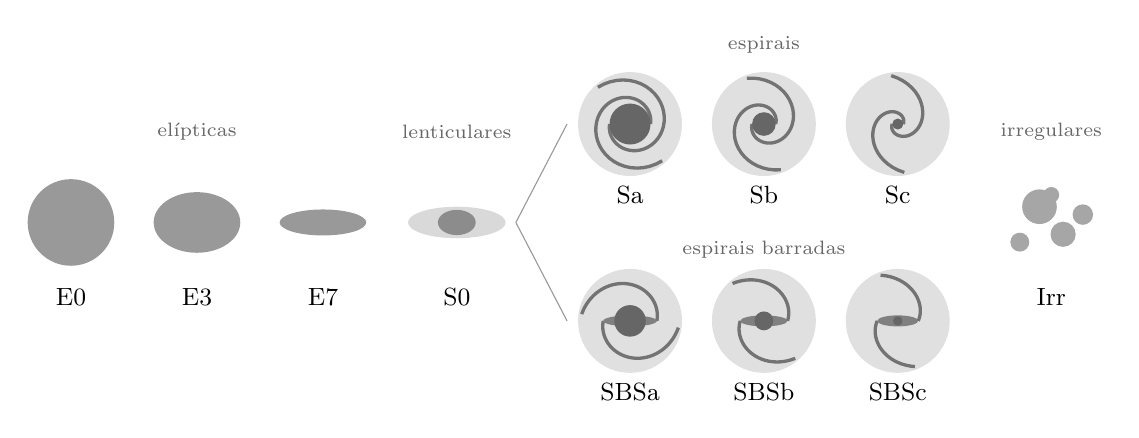
\begin{tikzpicture}[font=\small]
\def\spiralgal#1#2#3#4#5{% x, y, bulge radius, winding rate, bar half-length
  \begin{scope}[shift={(#1,#2)}]
    \fill[black!12] (0,0) circle (0.66);
    \pgfmathsetmacro{\rs}{max(#3,#5)}
    \pgfmathsetmacro{\th}{ln(0.62/\rs)/#4}
    \foreach \a in {0,180}
      \draw[line width=1.2pt, black!55, rotate=\a]
        plot[domain=0:\th, samples=40] ({\rs*exp(#4*\x)*cos(\x r)}, {\rs*exp(#4*\x)*sin(\x r)});
    \ifdim #5pt>0pt \fill[black!50] (0,0) ellipse (#5 and 0.07); \fi
    \fill[black!60] (0,0) circle (#3);
  \end{scope}}
\fill[black!40] (0,0) circle (0.55);
\fill[black!40] (1.6,0) ellipse (0.55 and 0.385);
\fill[black!40] (3.2,0) ellipse (0.55 and 0.165);
\fill[black!15] (4.9,0) ellipse (0.62 and 0.20);
\fill[black!45] (4.9,0) ellipse (0.24 and 0.16);
\draw[black!40] (5.65,0) -- (6.3,1.25);
\draw[black!40] (5.65,0) -- (6.3,-1.25);
\spiralgal{7.1}{1.25}{0.26}{0.16}{0}
\spiralgal{8.8}{1.25}{0.15}{0.28}{0}
\spiralgal{10.5}{1.25}{0.07}{0.45}{0}
\spiralgal{7.1}{-1.25}{0.20}{0.20}{0.34}
\spiralgal{8.8}{-1.25}{0.12}{0.32}{0.30}
\spiralgal{10.5}{-1.25}{0.06}{0.45}{0.26}
\foreach \p/\r in {(12.3,0.2)/0.22,(12.6,-0.15)/0.16,(12.05,-0.25)/0.12,(12.45,0.35)/0.1,(12.85,0.1)/0.13}
  \fill[black!35] \p circle (\r);
\foreach \x/\t in {0/E0,1.6/E3,3.2/E7,4.9/S0}
  \node at (\x,-0.95) {\t};
\foreach \x/\t in {7.1/Sa,8.8/Sb,10.5/Sc}
  { \node at (\x,0.35) {\t}; \node at (\x,-2.15) {SB\t}; }
\node at (12.45,-0.95) {Irr};
\node[font=\scriptsize, black!60] at (1.6,1.15) {elípticas};
\node[font=\scriptsize, black!60] at (4.9,1.15) {lenticulares};
\node[font=\scriptsize, black!60] at (8.8,2.25) {espirais};
\node[font=\scriptsize, black!60] at (8.8,-0.35) {espirais barradas};
\node[font=\scriptsize, black!60] at (12.45,1.15) {irregulares};
\end{tikzpicture}
\par\smallskip{\small A \omterm{def:b3:milky-way-galaxies:types}{sequência de Hubble} desenhada como um diapasão,
de forma esquemática. As elípticas são designadas pelo seu achatamento aparente;
o diapasão se bifurca nas lenticulares em espirais comuns e barradas,
ordenadas de bojos grandes e braços muito enrolados (a) a bojos pequenos e
braços abertos (c); as irregulares fecham a sequência.}\label{fig:b3:milky-way-galaxies:fork}
\end{omfigure}
% ledger: buta11:hubble

As classes descrevem formas vistas no céu, e um único rótulo esconde uma
faixa: uma elíptica vista ao longo do seu eixo mais curto parece redonda, qualquer que seja
seu achatamento real, e as fronteiras entre classes vizinhas são uma
questão de julgamento. Em um catálogo das galáxias próximas, a
Via Láctea é listada como S(B)bc, uma espiral entre Sb e Sc com barra; sua grande
vizinha Andrômeda (M31) é Sb, a galáxia do Triângulo (M33) é Sc, e
as Grande e Pequena Nuvens de Magalhães são irregulares.
% ledger: buta11:hubble, mcconn12:local-group

\begin{omfigure}
\centering
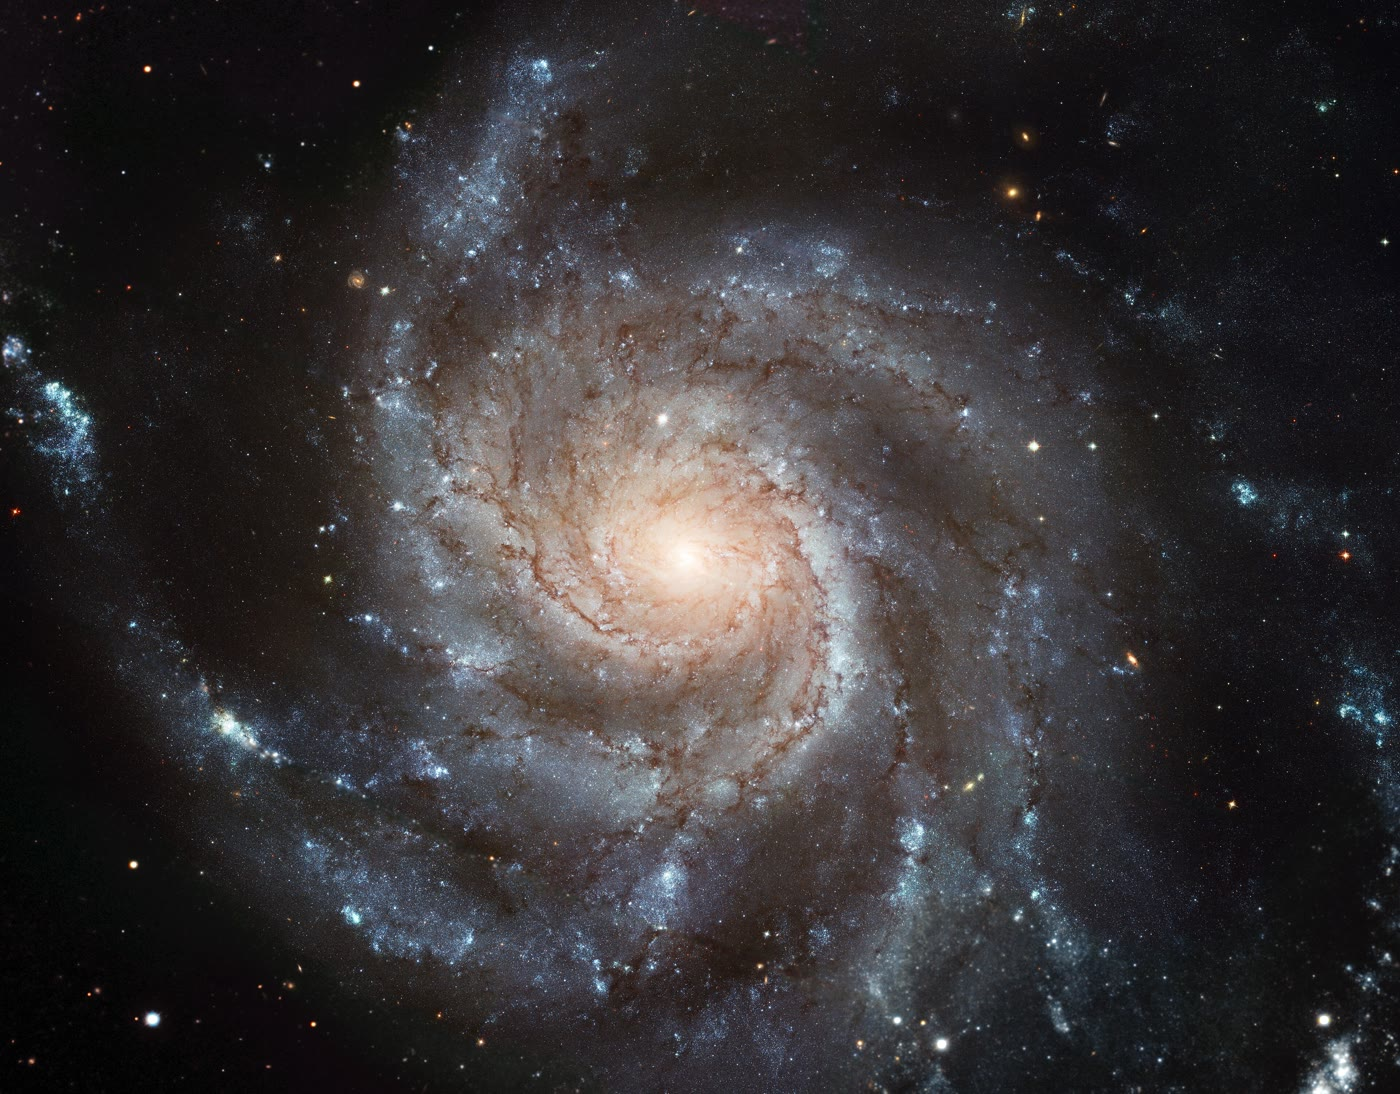
\includegraphics[width=0.66\linewidth]{images/book5/b3-m101.jpg}
\par\smallskip{\small A \omterm{def:b3:milky-way-galaxies:types}{galáxia espiral} M101, vista de frente pelo
Telescópio Espacial Hubble, em um mosaico de 51 exposições, recortado nas bordas: um bojo pequeno,
brilhante e amarelado; braços abertos, mais azulados e nodosos, com aglomerados de
estrelas jovens; faixas marrons de poeira ao longo dos braços. Imagem ESA e NASA
(Hubble, heic0602), CC BY~4.0.}\label{fig:b3:milky-way-galaxies:m101}
\end{omfigure}
% ledger: photo:b3-m101

Por que os braços espirais não se enrolam? Em um disco cuja \omterm{def:b3:milky-way-galaxies:rotation-curve}{curva de rotação} é plana,
uma estrela à metade da distância do centro dá uma volta na metade do tempo.
Uma espiral de estrelas se enrolaria mais apertada a cada volta, e depois de algumas voltas
do disco ela seria uma espiral cerrada (\cref{exo:b3:milky-way-galaxies:11}).

\begin{definition}[Teoria das ondas de densidade]\label{def:b3:milky-way-galaxies:density-wave}
A \emph{teoria das ondas de densidade}\index{teoria das ondas de densidade} explica os braços espirais
como uma onda de maior densidade em um disco, um padrão espiral que gira
rigidamente com sua própria velocidade angular, a velocidade do padrão, enquanto as estrelas e
o gás se movem através dele, desacelerando ao entrar no braço congestionado e
acelerando ao sair, como carros em um engarrafamento.
\end{definition}

A teoria, proposta em 1964, livra os braços do problema do enrolamento.
O gás que entra em um braço é comprimido, e estrelas se formam ali: os braços são
destacados por estrelas jovens e gás luminoso, enquanto as estrelas velhas se distribuem
de forma bem mais uniforme. Ainda se debate se os braços são ondas de longa duração;
simulações computacionais de discos com mais frequência produzem braços transitórios,
que se dissolvem e se reformam, e uma galáxia que passa ou uma barra podem induzir uma
espiral de dois braços.
% ledger: dobbs14:density-wave

\begin{definition}[Buraco negro supermassivo]\label{def:b3:milky-way-galaxies:smbh}
Um \emph{buraco negro supermassivo}\index{buraco negro supermassivo} é um buraco
negro de um milhão de massas solares ou mais no centro de uma galáxia.
\end{definition}

No centro da Galáxia, a fonte de rádio compacta Sagittarius~A*
(Sgr~A*) situa-se entre estrelas em órbitas apertadas e rápidas. Suas órbitas exigem uma
massa central de cerca de quatro milhões de sóis, $\num[separate-uncertainty=true]{4.2 \pm 0.2 e6}$
massas solares, segundo uma revisão das medições. A Sgr~A* quase não se move
em relação a galáxias distantes: retirado o movimento orbital do Sol, seu
movimento residual é de no máximo alguns quilômetros por segundo, logo ela retém ao
menos um quarto dessa massa. Seu tamanho é comparável ao seu raio de Schwarzschild,
e sua densidade, acima de \num{4e23} massas solares por parsec cúbico,
é muito próxima da esperada para um buraco negro: a evidência de
que a Sgr~A* é um buraco negro é esmagadora.
% ledger: reid20:sgra, bhg16:structure, gravity19:r0

\begin{definition}[Grupo Local; aglomerado de galáxias]\label{def:b3:milky-way-galaxies:groups}
O \emph{Grupo Local}\index{Grupo Local} é o grupo gravitacionalmente ligado
de galáxias dominado pela Via Láctea e por Andrômeda, cada uma com
suas galáxias satélites. Um \emph{aglomerado de galáxias}\index{aglomerado de galáxias} é
um dos maiores sistemas gravitacionalmente ligados: muitas galáxias mantidas,
com um gás quente que emite raios X, em um poço gravitacional comum,
formado sobretudo por matéria escura.
\end{definition}

Mais de cem galáxias estão a menos de \qty{3}{Mpc} do Sol, a maioria
delas anãs. A Grande Nuvem de Magalhães está a cerca de \qty{50}{kpc}, Andrômeda a
\qty{783}{kpc} e se aproximando de nós a \qty{300}{km.s^{-1}}, e os membros ligados
do grupo estão a cerca de \qty{1.06}{Mpc} de seu centro de
massa, entre a Galáxia e Andrômeda, onde se desprendem da
expansão do Universo. Sua massa, obtida a partir do movimento das duas grandes
galáxias uma em direção à outra, é da ordem de \num{5e12} massas solares. Em um
\omterm{def:b3:milky-way-galaxies:groups}{aglomerado de galáxias} massivo, o gás quente, a cerca de \qty{e8}{K}, contém cerca de dez
vezes a massa das estrelas; galáxias e gás juntos são leves demais para
a profundidade do poço gravitacional, e a maior parte da massa do aglomerado,
da ordem de \num{e15} massas solares, é escura.
% ledger: mcconn12:local-group, kravtsov12:clusters

\section{A escada de distâncias}\label{sec:b3:milky-way-galaxies:ladder}

Uma paralaxe fornece uma distância apenas pela geometria, mas as paralaxes diminuem com
a distância. O melhor catálogo delas mede uma paralaxe com uma
incerteza de 0.02 a \qty{0.03}{mas} para estrelas mais brilhantes que
magnitude~15, o que dá uma distância com incerteza de \qty{10}{\percent} até cerca de
\qty{4}{kpc}; a Grande Nuvem de Magalhães, a \qty{50}{kpc}, tem uma
paralaxe de \qty{0.02}{mas}. Mais além, as distâncias se apoiam em objetos cuja
luminosidade é conhecida.
% ledger: gaia:dr3, freedman19:trgb

\begin{definition}[Vela padrão; escada de distâncias]\label{def:b3:milky-way-galaxies:ladder}
Uma \emph{vela padrão}\index{vela padrão} é uma classe de objetos
cuja magnitude absoluta é conhecida ou pode ser inferida de uma propriedade
medida independentemente da distância, de modo que sua magnitude aparente forneça
seu módulo de distância. A \emph{escada de distâncias}\index{escada de distâncias} é
a cadeia de métodos, cada um calibrado com objetos próximos o bastante para serem
medidos também pelo método anterior, cadeia que leva as distâncias desde
as paralaxes até o Universo em expansão.
\end{definition}

\begin{definition}[Variável cefeida; lei de Leavitt]\label{def:b3:milky-way-galaxies:cepheid}
Uma \emph{variável cefeida}\index{variável cefeida} é uma estrela jovem, luminosa,
pulsante cujo brilho varia com um período estritamente regular,
de cerca de um dia a várias semanas. A \emph{lei de Leavitt}\index{lei de Leavitt},
ou relação período--luminosidade, é a relação linear entre a magnitude absoluta média
de uma cefeida e o logaritmo de seu período, com períodos mais longos
para as estrelas mais brilhantes.
\end{definition}

A relação foi descoberta na Pequena Nuvem de Magalhães, cujas estrelas
estão quase todas à mesma distância, em 1908. A poeira na galáxia que
hospeda uma cefeida a enfraquece e a avermelha; mas o enfraquecimento é maior no
visível do que no infravermelho próximo, em uma razão fixa para um dado tipo de
poeira, e a combinação $W_I = I - 1.55\,(V - I)$ das magnitudes nas
bandas I e V, o índice de Wesenheit, é escolhido de modo que o enfraquecimento
se cancele. A figura abaixo mostra isso para 2315 cefeidas da Grande
Nuvem de Magalhães: a \omterm{def:b3:milky-way-galaxies:cepheid}{lei de Leavitt} é uma reta bem definida, com dispersão de
\qty{0.078}{mag}, ou seja, \qty{3.6}{\percent} em distância para uma única
estrela.
% ledger: sos15:leavitt, data:b5-ogle-lmc-cep

\begin{omfigure}
\centering
\begin{tikzpicture}
\begin{axis}[width=0.80\linewidth, height=0.52\linewidth,
  xmin=-0.05, xmax=1.6, ymin=10, ymax=16.6, y dir=reverse,
  xlabel={$\log_{10}(P/\mathrm{d})$}, ylabel={Índice de Wesenheit $W_I$ (mag)},
  tick label style={font=\scriptsize}, label style={font=\small},
  legend style={font=\scriptsize, at={(0.5,-0.17)}, anchor=north, legend columns=3, draw=none, cells={anchor=west}, /tikz/every even column/.append style={column sep=1em}},
  legend image post style={scale=2.2}]
\addplot[only marks, mark=*, mark size=0.45pt, omDef, opacity=0.6] table[x=logp, y=w] {figdata/out/bachelor-3-distance_ladder-pl.dat};
\addlegendentry{Cefeidas}
\addplot[only marks, mark=x, mark size=1.6pt, red!70!black] table[x=logp, y=w] {figdata/out/bachelor-3-distance_ladder-clipped.dat};
\addlegendentry{excluídas ($>3\sigma$)}
\addplot[thick, black] table[x=logp, y=w_fit] {figdata/out/bachelor-3-distance_ladder-fit.dat};
\addlegendentry{ajuste}
\node[font=\scriptsize, anchor=south west, fill=white, inner sep=1pt] at (axis cs:0.55,11.0) {$W_I = -3.315\log_{10}P + 15.889$};
\end{axis}
\end{tikzpicture}
\par\smallskip{\small A \omterm{def:b3:milky-way-galaxies:cepheid}{lei de Leavitt} na Grande Nuvem de Magalhães:
o índice de Wesenheit de 2315 cefeidas pulsando em seu modo fundamental
em função do logaritmo de seus períodos (levantamento OGLE, Soszy\'nski e
outros, 2015, via o CDS). Estrelas mais brilhantes estão mais acima. Uma reta
ajustada por mínimos quadrados, após descartar 92 estrelas com mais de três
desvios-padrão em relação a ela, reproduz a relação publicada
($-3.314$, $15.888$). Com o módulo de distância da Nuvem, 18.477, a reta
fornece a magnitude absoluta de Wesenheit de qualquer cefeida a partir de seu período.}\label{fig:b3:milky-way-galaxies:leavitt}
\end{omfigure}
% ledger: data:b5-ogle-lmc-cep, sos15:leavitt, freedman19:trgb

\begin{definition}[Ponta do ramo das gigantes vermelhas]\label{def:b3:milky-way-galaxies:trgb}
A \emph{ponta do ramo das gigantes vermelhas}\index{ponta do ramo das gigantes vermelhas}
(TRGB) é o limite superior abrupto das luminosidades das gigantes vermelhas de
uma \omterm{def:b3:milky-way-galaxies:populations}{população estelar} antiga, fixado pela ignição do hélio em seus núcleos,
o flash do hélio; na banda I ela situa-se quase na mesma
magnitude absoluta em toda população antiga, $M_I \approx -4.05$ para a cor
$V - I = 1.6$, dependendo apenas fracamente da composição química.
\end{definition}

A ponta é medida nos halos esparsos das galáxias, onde há pouca poeira e pouca
aglomeração; ela usa estrelas velhas do halo onde as cefeidas usam estrelas
jovens do disco, e os dois métodos não compartilham física alguma. Cefeidas e a
TRGB alcançam algumas dezenas de megaparsecs, em galáxias onde explodiu uma
\omterm{def:b3:milky-way-galaxies:ladder}{vela padrão} rara e muito mais brilhante: uma supernova do tipo Ia, a explosão
termonuclear de uma anã branca, que o leitor recorda dos livros de física,
cuja magnitude absoluta de pico, uma vez corrigida pela
forma de sua curva de luz e por sua cor, é
$M_B = \qty[separate-uncertainty=true]{-19.253 \pm 0.027}{mag}$. Tais
supernovas são observadas a centenas de megaparsecs.
% ledger: freedman19:trgb, riess22:h0

\begin{definition}[Relação de Tully--Fisher]\label{def:b3:milky-way-galaxies:tully-fisher}
A \emph{relação de Tully--Fisher}\index{relação de Tully--Fisher} é a
correlação entre a luminosidade, ou melhor, a massa de estrelas e gás,
de uma \omterm{def:b3:milky-way-galaxies:types}{galáxia espiral} e a velocidade de sua \omterm{def:b3:milky-way-galaxies:rotation-curve}{curva de rotação} plana; em sua
forma bariônica, $M_\mathrm{b} = A\,V^4$, ela vale de cerca de 30 a
\qty{300}{km.s^{-1}}.
\end{definition}

O espectro de 21 cm de uma galáxia fornece sua velocidade máxima de rotação, a
relação fornece sua luminosidade, independentemente de sua distância, e seu
fluxo então fornece a distância: um degrau para galáxias espirais distantes demais para
estrelas isoladas. A Galáxia, por sua luminosidade e rotação, cai sobre a relação.
% ledger: mcgaugh00:btf, nrao:hi-line, bhg16:structure

\begin{omfigure}
\centering
\pgfplotstableread{figdata/out/bachelor-3-distance_ladder-ladder.dat}\laddertab
\pgfplotstableread{figdata/out/bachelor-3-distance_ladder-anchors.dat}\anchortab
\pgfplotstablegetelem{0}{d_hi}\of{\laddertab}\let\plxhi\pgfplotsretval
\pgfplotstablegetelem{1}{d_lo}\of{\laddertab}\let\cephlo\pgfplotsretval
\pgfplotstablegetelem{1}{d_hi}\of{\laddertab}\let\cephhi\pgfplotsretval
\pgfplotstablegetelem{3}{d_lo}\of{\laddertab}\let\snlo\pgfplotsretval
\pgfplotstablegetelem{3}{d_hi}\of{\laddertab}\let\snhi\pgfplotsretval
\pgfplotstablegetelem{1}{d}\of{\anchortab}\let\mthirtyone\pgfplotsretval
\pgfplotstablegetelem{2}{d}\of{\anchortab}\let\nfourtwo\pgfplotsretval
\begin{tikzpicture}
\begin{axis}[width=0.92\linewidth, height=0.42\linewidth,
  xmode=log, xmin=1e-3, xmax=2e6, ymin=0.4, ymax=4.9,
  ytick={1,2,3,4}, yticklabels={paralaxes, cefeidas, TRGB, SNe~Ia},
  xtick={1e-3,1e-2,1e-1,1,10,100,1e3,1e4,1e5,1e6},
  xticklabels={1\,pc,,,1\,kpc,,,1\,Mpc,,,1\,Gpc},
  xlabel={distância}, tick label style={font=\scriptsize}, label style={font=\small},
  y tick label style={font=\small}, axis y line*=left, axis x line*=bottom]
\draw[line width=7pt, omDef!70] (axis cs:1e-3,1) -- (axis cs:\plxhi,1);
\draw[line width=7pt, omMeth!70] (axis cs:\cephlo,2) -- (axis cs:\cephhi,2);
\draw[line width=7pt, omProp!70] (axis cs:\cephlo,3) -- (axis cs:\cephhi,3);
\draw[line width=7pt, red!60] (axis cs:\snlo,4) -- (axis cs:\snhi,4);
\draw[densely dotted, thick] (axis cs:\cephlo,0.4) -- (axis cs:\cephlo,4.55) node[anchor=south, font=\scriptsize] {LMC};
\draw[densely dotted, thick] (axis cs:\mthirtyone,0.4) -- (axis cs:\mthirtyone,4.55) node[anchor=south, font=\scriptsize] {M31};
\draw[densely dotted, thick] (axis cs:\nfourtwo,0.4) -- (axis cs:\nfourtwo,4.55) node[anchor=south, font=\scriptsize] {NGC~4258};
\draw[->, thick, black!60] (axis cs:\plxhi,1.25) to[out=30, in=200] (axis cs:\cephlo,1.75);
\draw[->, thick, black!60] (axis cs:\cephhi,2.25) to[out=40, in=220] (axis cs:\snlo,3.75);
\end{axis}
\end{tikzpicture}
\par\smallskip{\small Os degraus da \omterm{def:b3:milky-way-galaxies:ladder}{escada de distâncias}, com as
distâncias em que cada um é usado aqui: paralaxes do melhor catálogo,
com erro de \qty{10}{\percent}, até \qty{4}{kpc}; cefeidas e a TRGB desde a
Grande Nuvem de Magalhães até as hospedeiras das supernovas do tipo Ia mais
próximas, \qty{45}{Mpc}; as supernovas da expansão suave, com desvios para o
vermelho de 0.023 a 0.15 (\qtyrange{96}{616}{Mpc} para $H_0 = 73$). Pontilhado: duas âncoras da
escala das cefeidas com distâncias geométricas (binárias eclipsantes na
LMC, máseres de água orbitando o buraco negro de NGC~4258), e M31, a
espiral grande mais próxima. Setas: cada degrau é calibrado em objetos que o
degrau abaixo também mede, as cefeidas da Galáxia por suas paralaxes, as
supernovas de galáxias próximas pelas cefeidas e pela TRGB de suas
hospedeiras.}\label{fig:b3:milky-way-galaxies:ladder-rungs}
\end{omfigure}
% ledger: gaia:dr3, riess22:h0, freedman19:trgb, mcconn12:local-group

No topo da escada, as supernovas medem a expansão do
Universo. A lei de Hubble, que o leitor recorda dos livros de física, faz a
velocidade de recessão $cz$ de uma galáxia distante proporcional à sua distância $d$,
$cz = H_0 d$ para pequenos desvios para o vermelho $z$; a constante de Hubble $H_0$ é o
coeficiente angular, e as supernovas, com suas distâncias obtidas da escada, a fornecem.

\begin{definition}[Tensão de Hubble]\label{def:b3:milky-way-galaxies:tension}
A \emph{tensão de Hubble}\index{tensão de Hubble} é o desacordo entre o
valor da constante de Hubble medido localmente com a
\omterm{def:b3:milky-way-galaxies:ladder}{escada de distâncias} e o valor inferido do fundo cósmico de micro-ondas com o
modelo cosmológico padrão.
\end{definition}

\begin{dated}{2022}
As cefeidas das hospedeiras de 42 supernovas do tipo Ia, ancoradas nas
paralaxes da Gaia, nos máseres de NGC~4258 e nas binárias eclipsantes da
Grande Nuvem de Magalhães, dão
$H_0 = \qty[separate-uncertainty=true]{73.04 \pm 1.04}{km.s^{-1}.Mpc^{-1}}$.
A \omterm{def:b3:milky-way-galaxies:trgb}{ponta do ramo das gigantes vermelhas}, calibrando cerca de uma centena de
supernovas, deu em 2019 $H_0 = 69.8 \pm 0.8 \pm \qty{1.7}{km.s^{-1}.Mpc^{-1}}$
(estatístico e sistemático). O mapa do satélite Planck do fundo cósmico de
micro-ondas, lido com o modelo cosmológico padrão, implica
$H_0 = \qty[separate-uncertainty=true]{67.4 \pm 0.5}{km.s^{-1}.Mpc^{-1}}$.
O valor das cefeidas e o valor do fundo diferem por cinco
desvios-padrão; o valor da TRGB situa-se entre eles. A origem da
discrepância não é conhecida: um erro ainda não encontrado em um dos degraus,
ou física ausente no modelo.
\end{dated}
% ledger: riess22:h0, freedman19:trgb, planck18:h0

\begin{inthelab}[Um satélite astrométrico e seu catálogo]
O satélite Gaia varre o céu seguindo um padrão programado, de modo que cada
estrela é medida várias vezes ao longo da missão. No solo, as unidades de
coordenação de um consórcio de processamento de dados transformam essas
medições em uma posição, uma paralaxe e um movimento próprio para cada uma de
mais de um bilhão de fontes: dos pequenos deslocamentos de uma estrela no
céu, a paralaxe é a parte que se repete a cada ano, e o movimento próprio
é a parte que se acumula. Cada catálogo é divulgado com artigos que
descrevem seu processamento e sua validação, e toda distância nas figuras
desta seção que se apoia em uma paralaxe se apoia em um desses
catálogos.
\end{inthelab}

\begin{dated}{2022}
O terceiro catálogo do Gaia, divulgado em 13 de junho de 2022 a partir de 34
meses de observações, fornece posições, paralaxes e movimentos próprios para
cerca de 1.46~bilhão de fontes, de magnitude~3 a~21, e velocidades radiais
médias para 33~milhões de estrelas. Suas incertezas de paralaxe são de 0.02 a
\qty{0.03}{mas} para estrelas mais brilhantes que a magnitude~15, \qty{0.07}{mas} na
magnitude~17, e \qty{0.5}{mas} na magnitude~20.
\end{dated}
% ledger: gaia:dr3

\section{Exercícios}

\begin{exercise}[$\star$]\label{exo:b3:milky-way-galaxies:1}
O ano galáctico do Sol. (a)~Com $R_0 = \qty{8.178}{kpc}$ e
$V_0 = \qty{229}{km.s^{-1}}$, calcule o período da órbita do Sol em torno do
Centro Galáctico, em milhões de anos. (b)~Quantas voltas o Sol deu desde a
formação do Sistema Solar, há \qty{4.54}{Gyr}?
\end{exercise}

\begin{exercise}[$\star$]\label{exo:b3:milky-way-galaxies:2}
O movimento de reflexo de Sgr~A*. (a)~Um movimento próprio de \qty{1}{mas}
por ano a \qty{1}{kpc} equivale a uma velocidade transversal de \qty{1}{au} por ano:
exprima-a em quilômetros por segundo. (b)~Sgr~A*, suposto em repouso no Centro
Galáctico a \qty{8.178}{kpc}, desloca-se ao longo do plano galáctico em \qty{6.411}{mas}
por ano. Calcule a velocidade do Sol em torno do centro e compare-a com o valor de
revisão, \qty[separate-uncertainty=true]{248 \pm 3}{km.s^{-1}}. (c)~Subtraia o movimento
peculiar do Sol na direção de rotação, \qty{11}{km.s^{-1}}, e
compare com $V_0$ obtido da \omterm{def:b3:milky-way-galaxies:rotation-curve}{curva de rotação}.
\end{exercise}

\begin{exercise}[$\star$]\label{exo:b3:milky-way-galaxies:3}
Classificação das elípticas. (a)~As isofotas de uma \omterm{def:b3:milky-way-galaxies:types}{galáxia elíptica} têm
razão entre os eixos de 0.6: dê sua classe. (b)~Qual é a razão entre os eixos de uma E7?
(c)~Por que uma galáxia E0 pode ser um sistema achatado?
\end{exercise}

\begin{exercise}[$\star$]\label{exo:b3:milky-way-galaxies:4}
Âncoras. Calcule as distâncias da Grande Nuvem de Magalhães
($\mu = 18.477$), de Andrômeda ($\mu = 24.47$) e de NGC~4258
($\mu = 29.398$). Que paralaxe teria uma estrela da Nuvem, e por que a
distância da Nuvem não pode ser medida por paralaxes?
\end{exercise}

\begin{exercise}[$\star\star$]\label{exo:b3:milky-way-galaxies:5}
A partir das \omterm{def:b3:milky-way-galaxies:rotation-curve}{constantes de Oort} $A = \qty{15.3}{km.s^{-1}.kpc^{-1}}$ e
$B = \qty{-11.9}{km.s^{-1}.kpc^{-1}}$: (a)~calcule a velocidade angular do
\omterm{def:b3:milky-way-galaxies:lsr}{padrão local de repouso} e, com $R_0 = \qty{8.178}{kpc}$, a velocidade circular $V_0$;
(b)~calcule a inclinação da \omterm{def:b3:milky-way-galaxies:rotation-curve}{curva de rotação} no Sol. (c)~Compare
com a \omterm{def:b3:milky-way-galaxies:rotation-curve}{curva de rotação} das gigantes vermelhas ($V_0 = \qty{229.0}{km.s^{-1}}$,
inclinação \qty{-1.7}{km.s^{-1}} por quiloparsec) e sugira por que as duas
diferem, dado que a mesma medição encontrou $C$ e $K$ não nulos.
\end{exercise}

\begin{exercise}[$\star\star$]\label{exo:b3:milky-way-galaxies:6}
Uma \omterm{def:b3:milky-way-galaxies:rotation-curve}{curva de rotação} plana e a densidade local. (a)~Para uma galáxia esférica
com \omterm{def:b3:milky-way-galaxies:rotation-curve}{curva de rotação} plana em \qty{229}{km.s^{-1}}, calcule a densidade a
\qty{8.178}{kpc}, em massas solares por parsec cúbico
($G = \qty{4.301e-6}{kpc.(km.s^{-1})^2}$ por massa solar). (b)~Mostre que
uma massa solar por parsec cúbico equivale a \qty{37.96}{GeV.cm^{-3}}, e exprima
a densidade local de matéria escura, \qty{0.30}{GeV.cm^{-3}}, em massas solares
por parsec cúbico. (c)~Por que a densidade de (a) é maior?
\end{exercise}

\begin{exercise}[$\star\star$]\label{exo:b3:milky-way-galaxies:7}
Uma distância por cefeida. Em uma \omterm{def:b3:milky-way-galaxies:types}{galáxia espiral} inventada, uma cefeida de
período \qty{30}{d} tem índice de Wesenheit médio $W_I = \qty{25.00}{mag}$.
(a)~Usando a \omterm{def:b3:milky-way-galaxies:cepheid}{lei de Leavitt} da Grande Nuvem de Magalhães,
$W_I = -3.314\log_{10}P + 15.888$, e o módulo de distância da Nuvem
18.477, calcule a magnitude de Wesenheit absoluta da cefeida. (b)~Calcule
a distância da galáxia. (c)~A dispersão da lei é \qty{0.077}{mag}: qual é
o erro relativo de distância a partir de uma cefeida, e a partir de cinquenta?
\end{exercise}

\begin{exercise}[$\star\star$]\label{exo:b3:milky-way-galaxies:8}
Uma distância pelo TRGB. No halo de uma galáxia inventada, a \omterm{def:b3:milky-way-galaxies:trgb}{ponta do ramo das
gigantes vermelhas} é encontrada em $I = \qty{26.00}{mag}$; a poeira ao longo da linha de
visada atenua a banda I em \qty{0.05}{mag}. Com $M_I = -4.05$, calcule o
módulo de distância e a distância. O que significa, em distância, uma incerteza de
\qty{0.04}{mag} na ponta?
\end{exercise}

\begin{exercise}[$\star\star$]\label{exo:b3:milky-way-galaxies:9}
A constante de Hubble a partir de supernovas. Para uma supernova da expansão
suave, $\log_{10}(cz) - 0.2\,m_B = a_B$, o intercepto do
diagrama de Hubble das supernovas, e o módulo de distância é
$m_B - M_B = 5\log_{10}(d/\mathrm{Mpc}) + 25$. (a)~Mostre que
$\log_{10}H_0 = 0.2\,M_B + a_B + 5$ ($H_0$ em quilômetros por segundo por
megaparsec). (b)~Com $M_B = -19.253$ e $a_B = 0.714158$, calcule $H_0$.
(c)~Qual $M_B$ daria $H_0 = \qty{67.4}{km.s^{-1}.Mpc^{-1}}$? Em quantas
magnitudes, e em que fração das distâncias, as duas
calibrações diferem?
\end{exercise}

\begin{exercise}[$\star\star\star$]\label{exo:b3:milky-way-galaxies:10}
De onde vem a lei de Tully--Fisher. (a)~Uma galáxia de disco de massa $M$
e raio $R$ gira com velocidade $V$: mostre que $M \approx RV^2/G$. (b)~Se todas
as galáxias espirais tivessem a mesma densidade superficial média $\Sigma = M/(\pi R^2)$,
mostre que $M \propto V^4$. (c)~Duas galáxias inventadas, sobre a mesma relação bariônica,
giram a 100 e \qty{229}{km.s^{-1}}: qual é a razão entre
suas massas? (d)~Duas galáxias giram com a mesma velocidade e têm a mesma
luminosidade; uma delas tem quatro vezes o fluxo da outra. Compare suas
distâncias.
\end{exercise}

\begin{exercise}[$\star\star\star$]\label{exo:b3:milky-way-galaxies:11}
O problema do enrolamento. Um disco gira com \omterm{def:b3:milky-way-galaxies:rotation-curve}{curva de rotação} plana a
\qty{229}{km.s^{-1}}. (a)~Converta esta velocidade para quiloparsecs por bilhão
de anos. (b)~Um braço reto de estrelas se estende, no instante zero, de 4 a
\qty{12}{kpc}. Calcule os períodos orbitais nas duas extremidades. (c)~Após
\qty{1}{Gyr}, de que ângulo a extremidade interna avançou em relação à
extremidade externa? Quantas voltas de espiral isso corresponde, e qual seria o aspecto do braço?
(d)~Como uma onda de densidade evita isso?
\end{exercise}

\begin{exercise}[$\star\star\star$]\label{exo:b3:milky-way-galaxies:12}
O buraco negro no centro. Tome a massa central como
\num{4.2e6} massas solares e $R_0 = \qty{8178}{pc}$. (a)~A estrela S2
orbita-o em \num{16}~anos: calcule o semieixo maior de sua órbita em
unidades astronômicas (terceira lei de Kepler em unidades solares, $a^3 = MP^2$ com
$a$ em au, $P$ em anos e $M$ em massas solares) e seu tamanho angular visto
da Terra. (b)~Calcule o raio de Schwarzschild do buraco negro em
metros e em unidades astronômicas, e o ângulo que seu diâmetro
subentende da Terra, em microssegundos de arco. (c)~Calcule a densidade média
da massa dentro de seu raio de Schwarzschild, em massas solares por
parsec cúbico, e compare-a com o limite inferior definido pelo movimento de Sgr~A*,
\num{4e23} massas solares por parsec cúbico.
\end{exercise}

\section{Problema: pesando a Galáxia}

\begin{problem}[{Problema de fim de semana --- a partir dos movimentos das estrelas e do gás até
a matéria escura dentro de \qty{20}{kpc}}]
\label{pb:b3:milky-way-galaxies:1}
Tome $R_0 = \qty{8.18}{kpc}$, $G = \qty{4.301e-6}{kpc.(km.s^{-1})^2}$ por
massa solar, e \qty{4.74}{km.s^{-1}} para um movimento próprio de
\qty{1}{mas} por ano a \qty{1}{kpc}. Todas as velocidades são relativas ao
LSR. Use os teoremas de Oort e do ponto tangente do capítulo, e a
aproximação esférica $M = RV^2/G$ para massas dinâmicas.

\medskip\noindent\textbf{Parte I --- A rotação local.} Um levantamento inventado
de estrelas do red clump, todas a $d = \qty{1.00}{kpc}$ no
plano galáctico, fornece uma velocidade radial média de \qty{+15.4}{km.s^{-1}} em
$\ell = \ang{45}$ e \qty{-15.2}{km.s^{-1}} em $\ell = \ang{135}$, e
movimentos próprios médios em longitude de \qty{-5.91}{mas} por ano em
$\ell = \ang{90}$ e \qty{+0.55}{mas} por ano em $\ell = \ang{0}$.
\begin{enumerate}
\item O que a fórmula de Oort prevê para as velocidades radiais em
  $\ell = \ang{45}$, \ang{90}, \ang{135} e \ang{180}?
\item Calcule $A$ a partir das duas velocidades radiais.
\item Calcule $B$ a partir do movimento próprio em $\ell = \ang{90}$.
\item Calcule $B$ novamente a partir do movimento próprio em $\ell = \ang{0}$, e
  compare.
\item Calcule a velocidade angular do LSR e a velocidade circular
  $V_0$.
\item Calcule a inclinação da \omterm{def:b3:milky-way-galaxies:rotation-curve}{curva de rotação} no Sol. A curva é
  crescente, plana ou decrescente?
\item Calcule o período da órbita do Sol e o número de voltas em
  \qty{4.54}{Gyr}.
\end{enumerate}

\medskip\noindent\textbf{Parte II --- A curva de rotação interna.} Tome
$V_0 = \qty{229}{km.s^{-1}}$. As maiores velocidades radiais nos
perfis de 21 cm em $\ell = \ang{40}$, \ang{50}, \ang{60} e \ang{70} são
82.9, 55.6, 32.4 e \qty{14.9}{km.s^{-1}}.
\begin{enumerate}[resume]
\item Por que o método do ponto tangente precisa de $\ang{0} < \ell < \ang{90}$
  (ou do quadrante espelhado), e por que ele falha além do círculo solar?
\item Calcule o raio do ponto tangente para cada longitude.
\item Calcule $V(R)$ em cada ponto tangente.
\item De quanto, em quilohertz, a linha do gás no ponto tangente
  em $\ell = \ang{40}$ está deslocada de sua frequência de repouso,
  \qty{1420.405751}{MHz}, e em que sentido?
\item Compare com a curva das gigantes vermelhas, que fornece \qty{226.8}{km.s^{-1}}
  em \qty{5.27}{kpc} e \qty{229.6}{km.s^{-1}} em \qty{7.22}{kpc}. A
  curva interna é crescente, plana ou decrescente?
\item Se a velocidade no ponto tangente em $\ell = \ang{40}$ fosse a de
  uma massa pontual no centro levando o Sol a $V_0$, qual seria ela?
  O que a comparação diz sobre a distribuição da massa?
\end{enumerate}

\medskip\noindent\textbf{Parte III --- A massa visível.} Use o modelo de massa
do capítulo, em unidades de massas solares e quiloparsecs: um
bojo de Plummer $M = \num{1.067e10}$, $b = 0.3$; um disco fino de Miyamoto--Nagai
$M = \num{3.944e10}$, $a = 5.3$, $b = 0.25$; um \omterm{def:b3:milky-way-galaxies:structure}{disco espesso} de mesma
massa com $a = 2.6$, $b = 0.8$.
\begin{enumerate}[resume]
\item Calcule a massa visível total do modelo e compare-a com o
  valor de revisão da massa estelar da Galáxia, \qty[separate-uncertainty=true]{5 \pm 1 e10}{} massas
  solares.
\item Calcule a velocidade circular só do bojo a \qty{20}{kpc}.
\item Calcule as do disco fino e as do \omterm{def:b3:milky-way-galaxies:structure}{disco espesso} a \qty{20}{kpc}.
\item Calcule a velocidade circular de toda a massa visível a
  \qty{20}{kpc}.
\item Calcule o mesmo em $R_0$ e compare com $V_0$.
\item Se toda a massa visível estivesse concentrada no centro, qual seria
  a velocidade a \qty{20}{kpc}? Por que o valor do modelo fica próximo dela?
\end{enumerate}

\medskip\noindent\textbf{Parte IV --- A matéria escura.} As gigantes vermelhas
fornecem uma velocidade circular de \qty{200}{km.s^{-1}} a \qty{20}{kpc}.
\begin{enumerate}[resume]
\item Calcule a massa dinâmica dentro de \qty{20}{kpc}.
\item Calcule a massa dinâmica da matéria visível dentro de
  \qty{20}{kpc}.
\item Calcule a massa de matéria escura dentro de \qty{20}{kpc} e mostre que
  sua fração é $1 - (V_\mathrm{vis}/V)^2$.
\item O halo NFW ajustado à curva inteira tem
  $\rho_0 = \num{1.06e7}$ massas solares por quiloparsec cúbico e
  $R_s = \qty{14.8}{kpc}$. Calcule sua massa dentro de \qty{20}{kpc} e a
  fração de matéria escura que ele implica. Por que ela difere da resposta anterior?
\item Calcule a densidade desse halo em $R_0$, em massas solares por
  parsec cúbico e em \unit{GeV.cm^{-3}} (uma massa solar por parsec cúbico
  equivale a \qty{37.96}{GeV.cm^{-3}}).
\item Dê a fração de matéria escura da massa dentro de \qty{20}{kpc}
  obtida a partir da velocidade medida, em por cento, com dois algarismos
  significativos.
\end{enumerate}
\end{problem}
% ledger: gravity19:r0, eilers19:table1, pouliasis17:model1, eilers19:halo, bhg16:structure, nrao:hi-line, const:G, const:au, iau:parsec, usgs:age-earth
